\documentclass[11pt]{article}
\usepackage{amsmath, amssymb, amscd, amsthm, amsfonts}
\usepackage{graphicx}
\usepackage{subcaption}
\usepackage{listings}
\usepackage{color}

\oddsidemargin 0pt
\evensidemargin 0pt
\marginparwidth 40pt
\marginparsep 10pt
\topmargin -20pt
\headsep 10pt
\textheight 8.7in
\textwidth 6.65in
\linespread{1.2}

\usepackage{imakeidx}
\usepackage[toc,page]{appendix}


\begin{document}

\section{ExB Drift}
\subsection{Soluzione analitica}
Ora consideriamo il moto di una particella in moto in presenza anche di un campo elettrico $\mathbf{E}$ oltre al campo magnetico $\mathbf{B}$. \\ 
$$\mathbf{B}=(0,0,B_z)    $$
$$\mathbf{E}=(0,E_y,0)  $$
Posso scrivere la $\mathbf{v}$ della particella come somma di una componente parallela e una perpendicolare a $\mathbf{B}$: 
$\mathbf{v} = \mathbf{v_{\parallel}} + \mathbf{v_{\perp}}$. \\
A sua volta $\mathbf{v_{\parallel}} = \mathbf{v_d} + \mathbf{v_g}(t)$
assumendo che la velocitá di drift sia costante nel tempo.
L'idea é quella di ricondurci a un moto piú semplice effettuando un cambio di sistema di riferimento.
Infatti, posso riscrivere (1) come:
$$ 
\frac{d\mathbf{v_g}}{dt} = \mathbf{E} + (\mathbf{v_d} + \mathbf{v_g}) \times \mathbf{B}$$
$$
\frac{d\mathbf{v_g}}{dt} = \left(\mathbf{E} + \mathbf{v_d} \times \mathbf{B}\right) + \mathbf{v_g} \times \mathbf{B}
$$
Posso annullare il termine con il campo elettrico imponendo una determinata $\mathbf{v_d}$:
$$
\mathbf{E} + \mathbf{v_d} \times \mathbf{B} = 0
$$
Applico il rotore a entrambi i membri e usando un' identitá vettoriale, ottengo:
$$
\mathbf{v_d} = \frac{\mathbf{E} \times \mathbf{B}}{\|\mathbf{B}\|^2}
$$
Mi sono spostato su un sistema di riferimento il cui campo $\mathbf{E}$ é nullo, per cui ritrovo un semplice moto di girazione:
$$
\frac{d\mathbf{v_g}}{dt} = \mathbf{v_g} \times \mathbf{B}
$$
Se considero $\mathbf{B}=(0,0,B_z)$ e $\mathbf{E}=(0,E_y,0)$ avró:
$$
\mathbf{v_d} = \frac{\mathbf{E} \times \mathbf{B}}{\|\mathbf{B}\|^2} = \frac{E_y}{B_z} \vec{i}
$$  
Posso riscrivere l'equazioni del moto come:
$$
\begin{cases} 
\frac{d(v_x - v_d)}{dt}=v_y B_z \\ 
\frac{dv_y}{dt}=-(v_x - v_d)B_z + E_y  \\ 
\frac{dv_z}{dt}=0 
\end{cases}
$$
La cui soluzione sará:
$$
\begin{cases}
v_x = \frac{E_y}{B_z} (1 + \cos(t)) \\
v_y = - \frac{E_y}{B_z}\sin(t) \\
v_z = 0 
\end{cases}
$$


La traiettoria della particella é una cicloide lungo la direzione x. Il moto è inaspettato avendo un campo elettrico agente lungo $y$, infatti ci aspetteremmo che la particella accelleri lungo questa direzione.\\
In realt\`a, quando la velocit\`a della particella aumenta cresce anche la forza risultante dall'interazione con $\mathbf{B}$, sempre normale alla traiettoria.
Infatti la carica ferma nell'origine subisce un accelerazione lungo y dovuta a $\mathbf{E}$. Appena la carica inizia a muoversi la forza magnetica agisce nella direzione normale alla traiettoria. Questo fino alla fine del periodo dove la forza risultante è nulla, per cui la carica si ferma e il moto si ripete periodico.\\


\subsection{Convergenza degli integratori}

Nel caso precedente di girazione abbiamo studiato le proprietá di conservazione dell'energia dei tre integratori, ora vorremmo studiarne le proprietá di convergenza.
Per fare ció confronteró la soluzione analitica trovata nella sezione precedente con la soluzione numerica. Questo verrá ripetuto per differenti timestep $dt$.
Come valori per $\mathbf{E}$, $\mathbf{B}$ e $\mathbf{v_0}$ della particella useremo:
$$\mathbf{B}=(0,0,1) $$
$$\mathbf{E}=(0,\frac{1}{2},0) $$
$$\mathbf{v_0} = (1,0,0)$$
\begin{figure}[ht]
  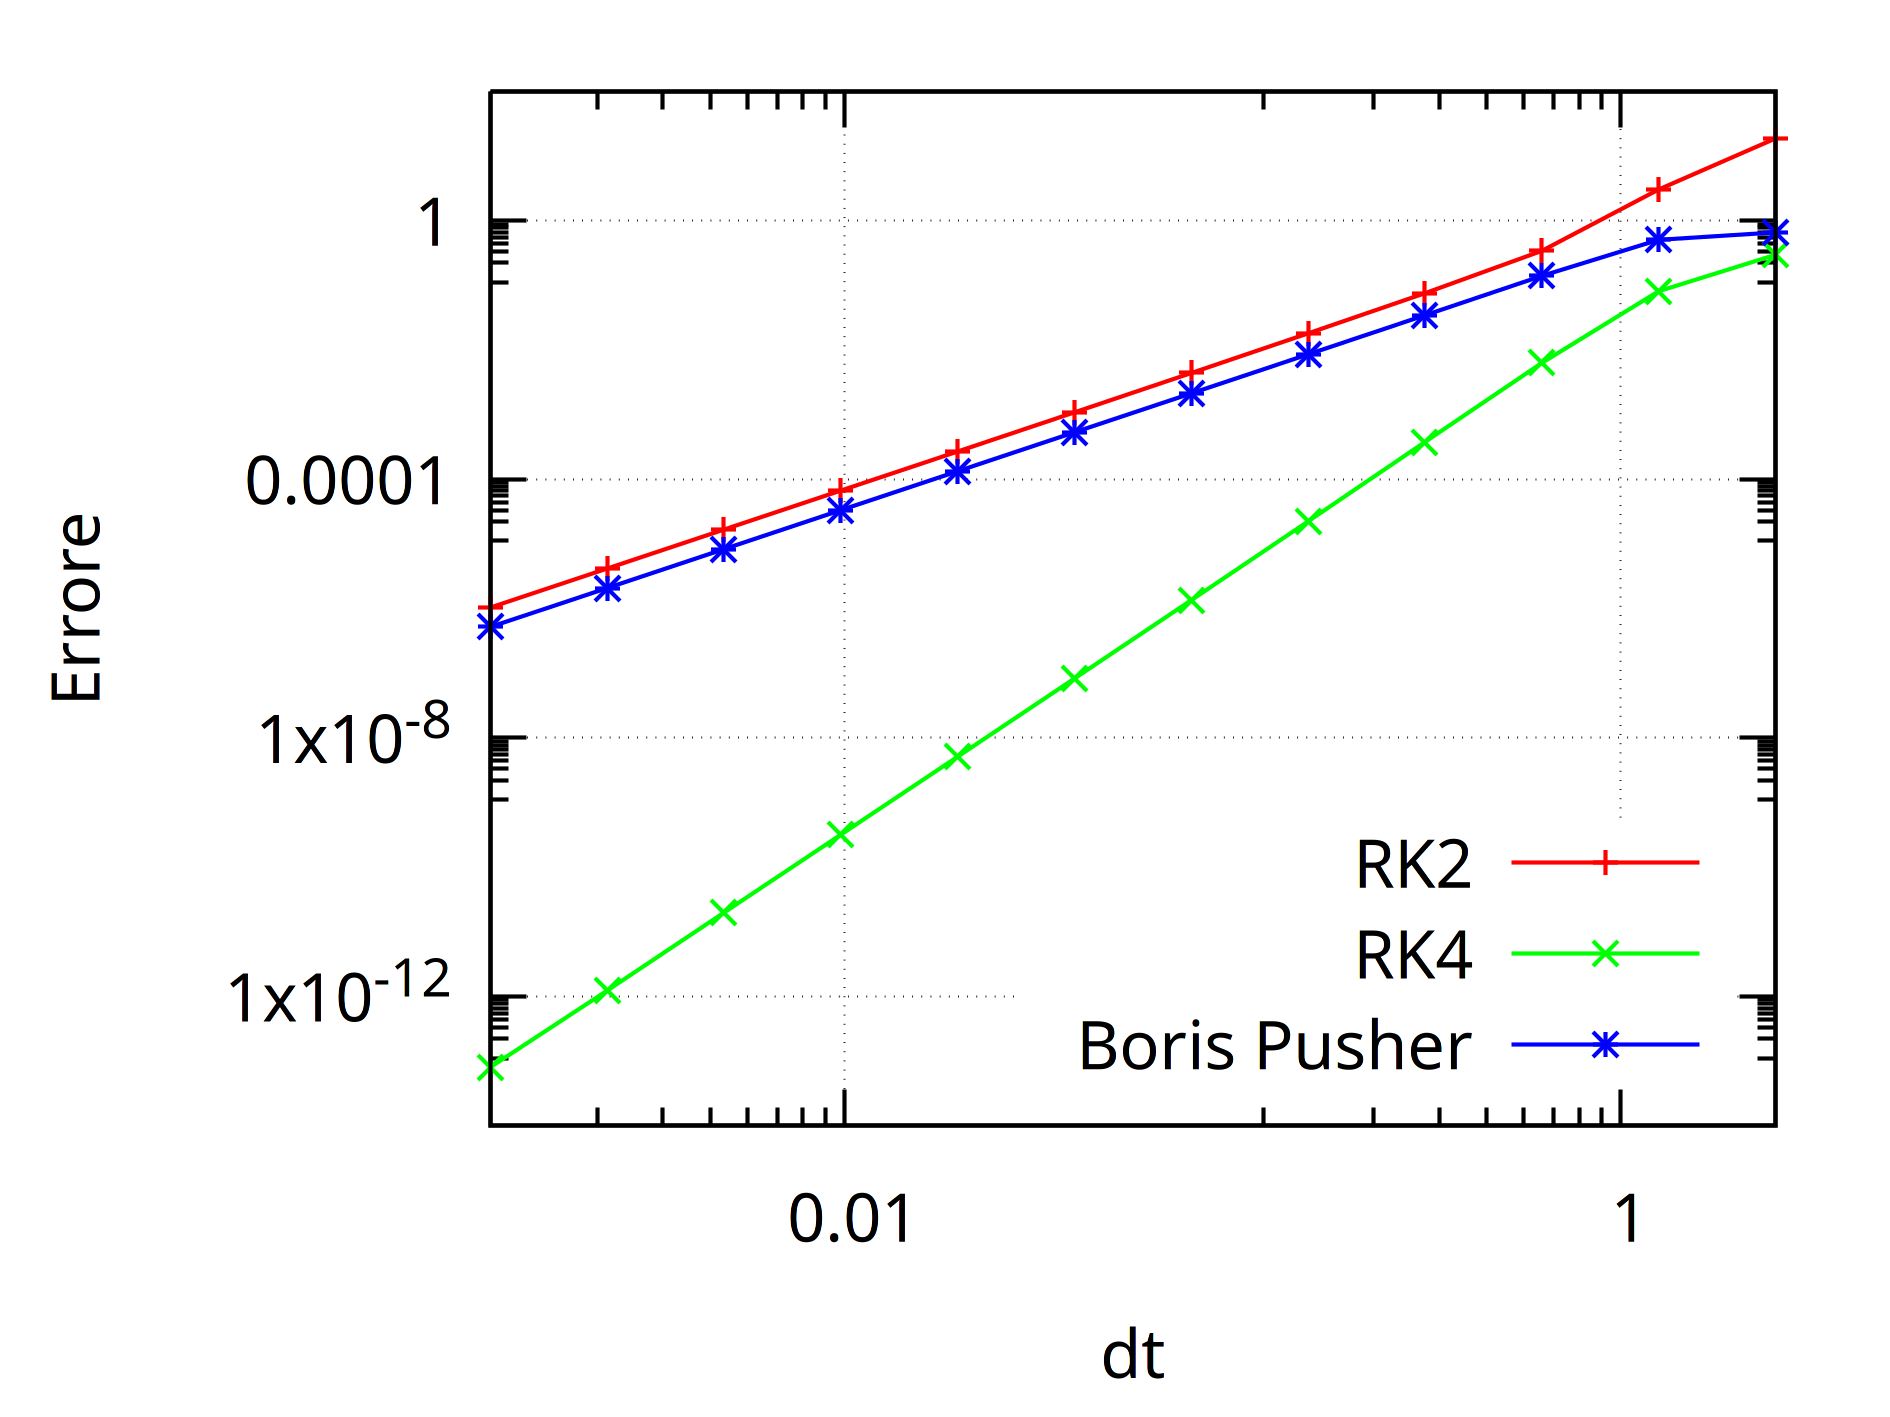
\includegraphics[width=.9\linewidth]{img/convergenza.png}  
  \caption{Errore al variare del timestep $dt$}
\end{figure}%

Verifichiamo come RK2 e Boris Pusher siano integratori del $2^o$ ordine: un fattore 10 per $dt$ comporta una riduzione di 100 nell'errore. RK4 é del $4^o$ ordine per cui a un fattore 10 del dt corrisponde una riduzione di $10^4$ per l'errore.

\newpage
\subsection{Soluzione Numerica}
Come integratore usiamo Boris Pusher,in quanto nonostante una minore precisione rispetto a RK4 otteniamo un' accuratezza sufficiente: $10^{-4}$ con timestep $dt = 10^{-2}$.\\
Come valori per $\mathbf{E}$, $\mathbf{B}$ e $\mathbf{v_0}$ della particella useremo:
$$\mathbf{B}=(0,0,1) $$
$$\mathbf{E}=(0,\frac{1}{2},0) $$
$$\mathbf{v_0} = (1,0,0)$$
\begin{figure}[ht]
\begin{subfigure}{.5\textwidth}
  \centering
  % include first image
  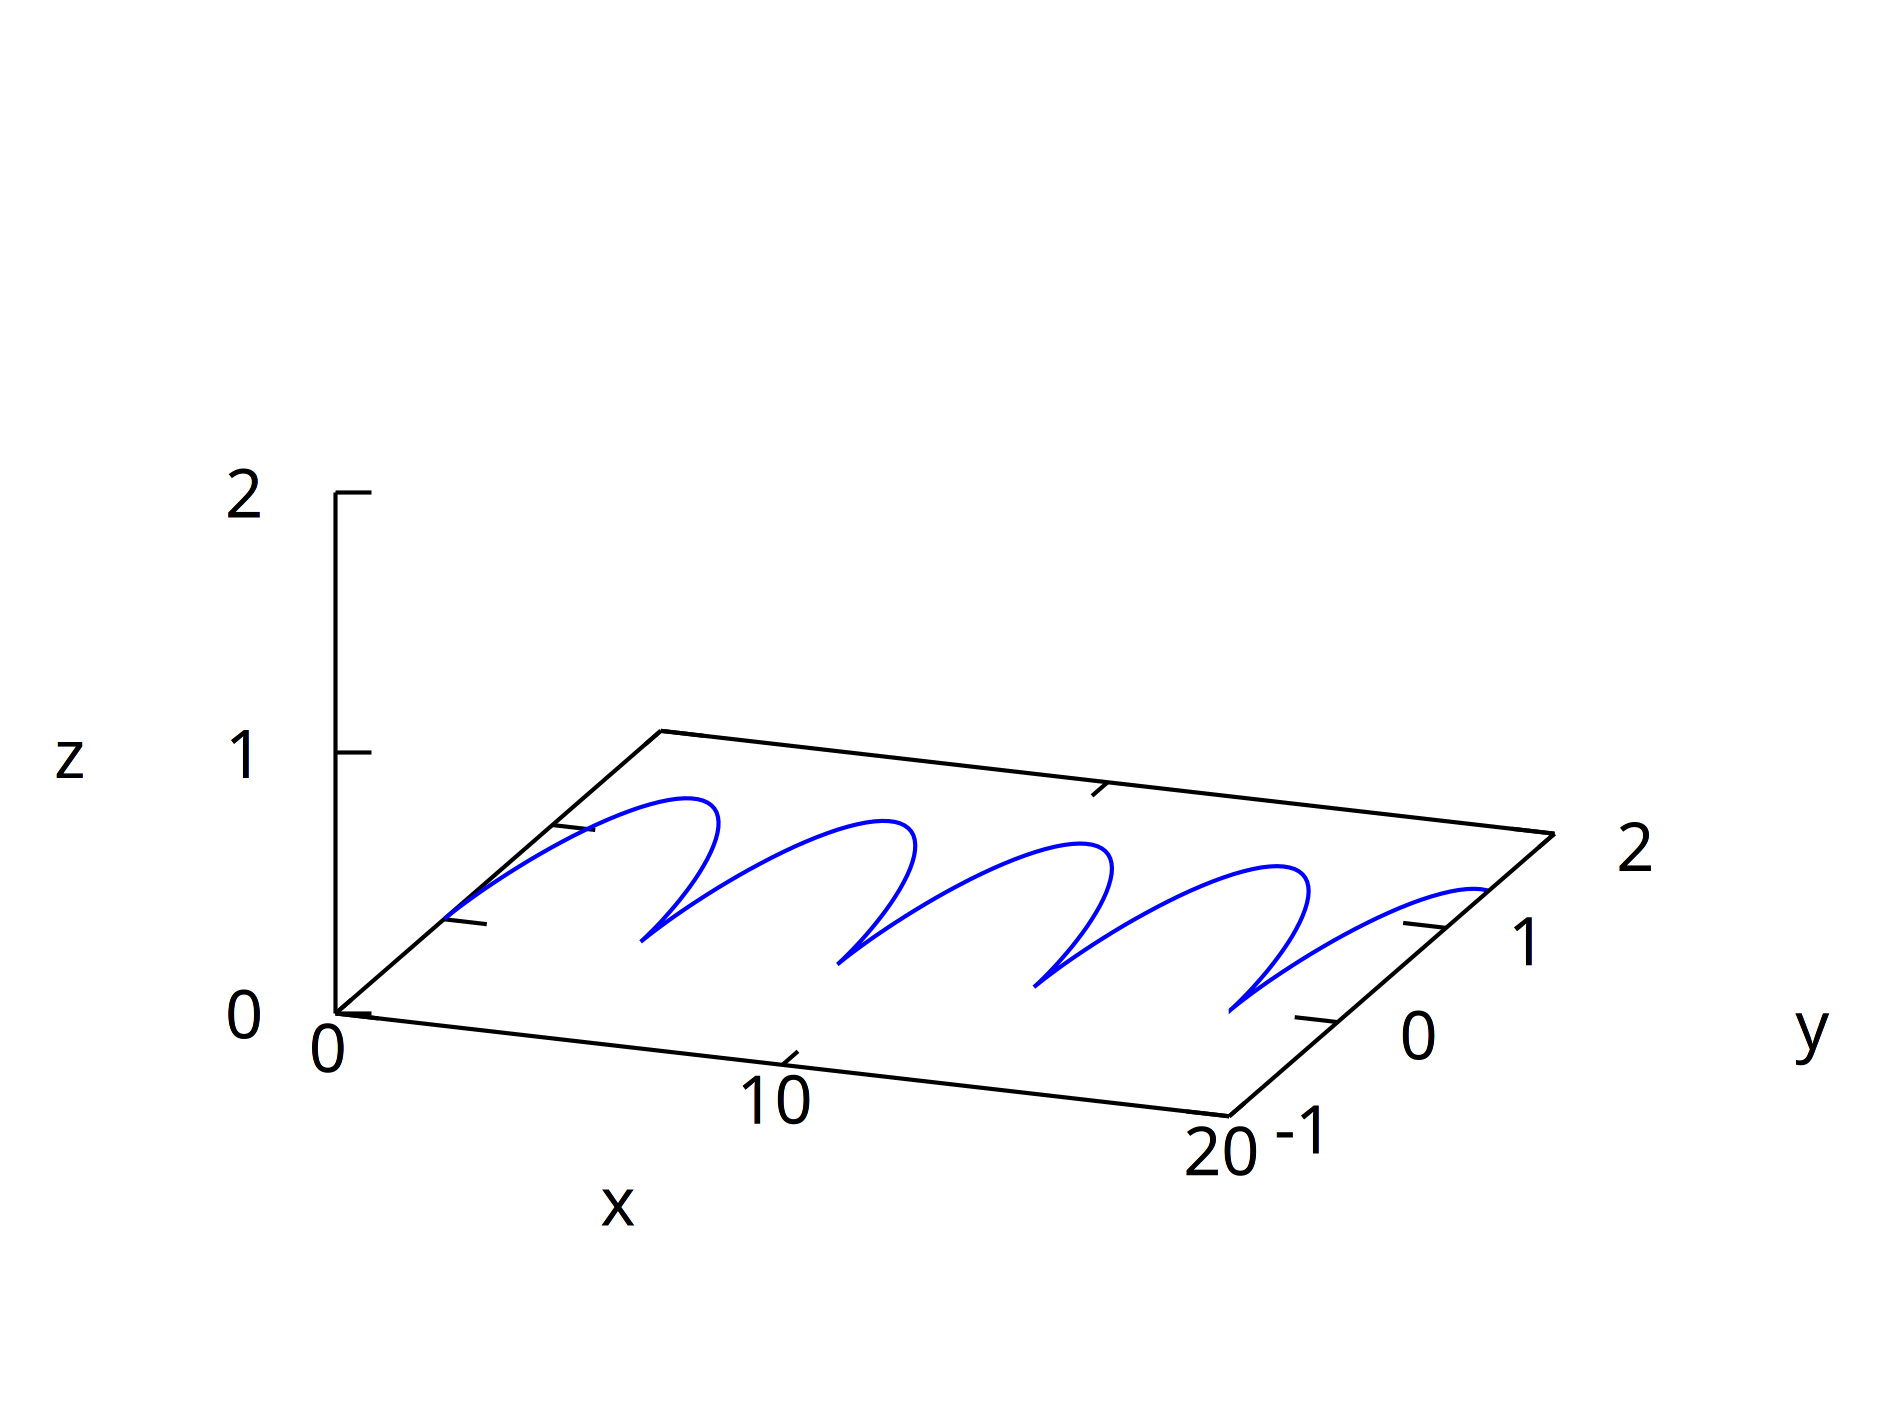
\includegraphics[width=.9\linewidth]{img/3dposizionedrift.png}  
  \caption{Traiettoria nello spazio 3d}
\end{subfigure}
\begin{subfigure}{.5\textwidth}
  \centering
  % include second image
  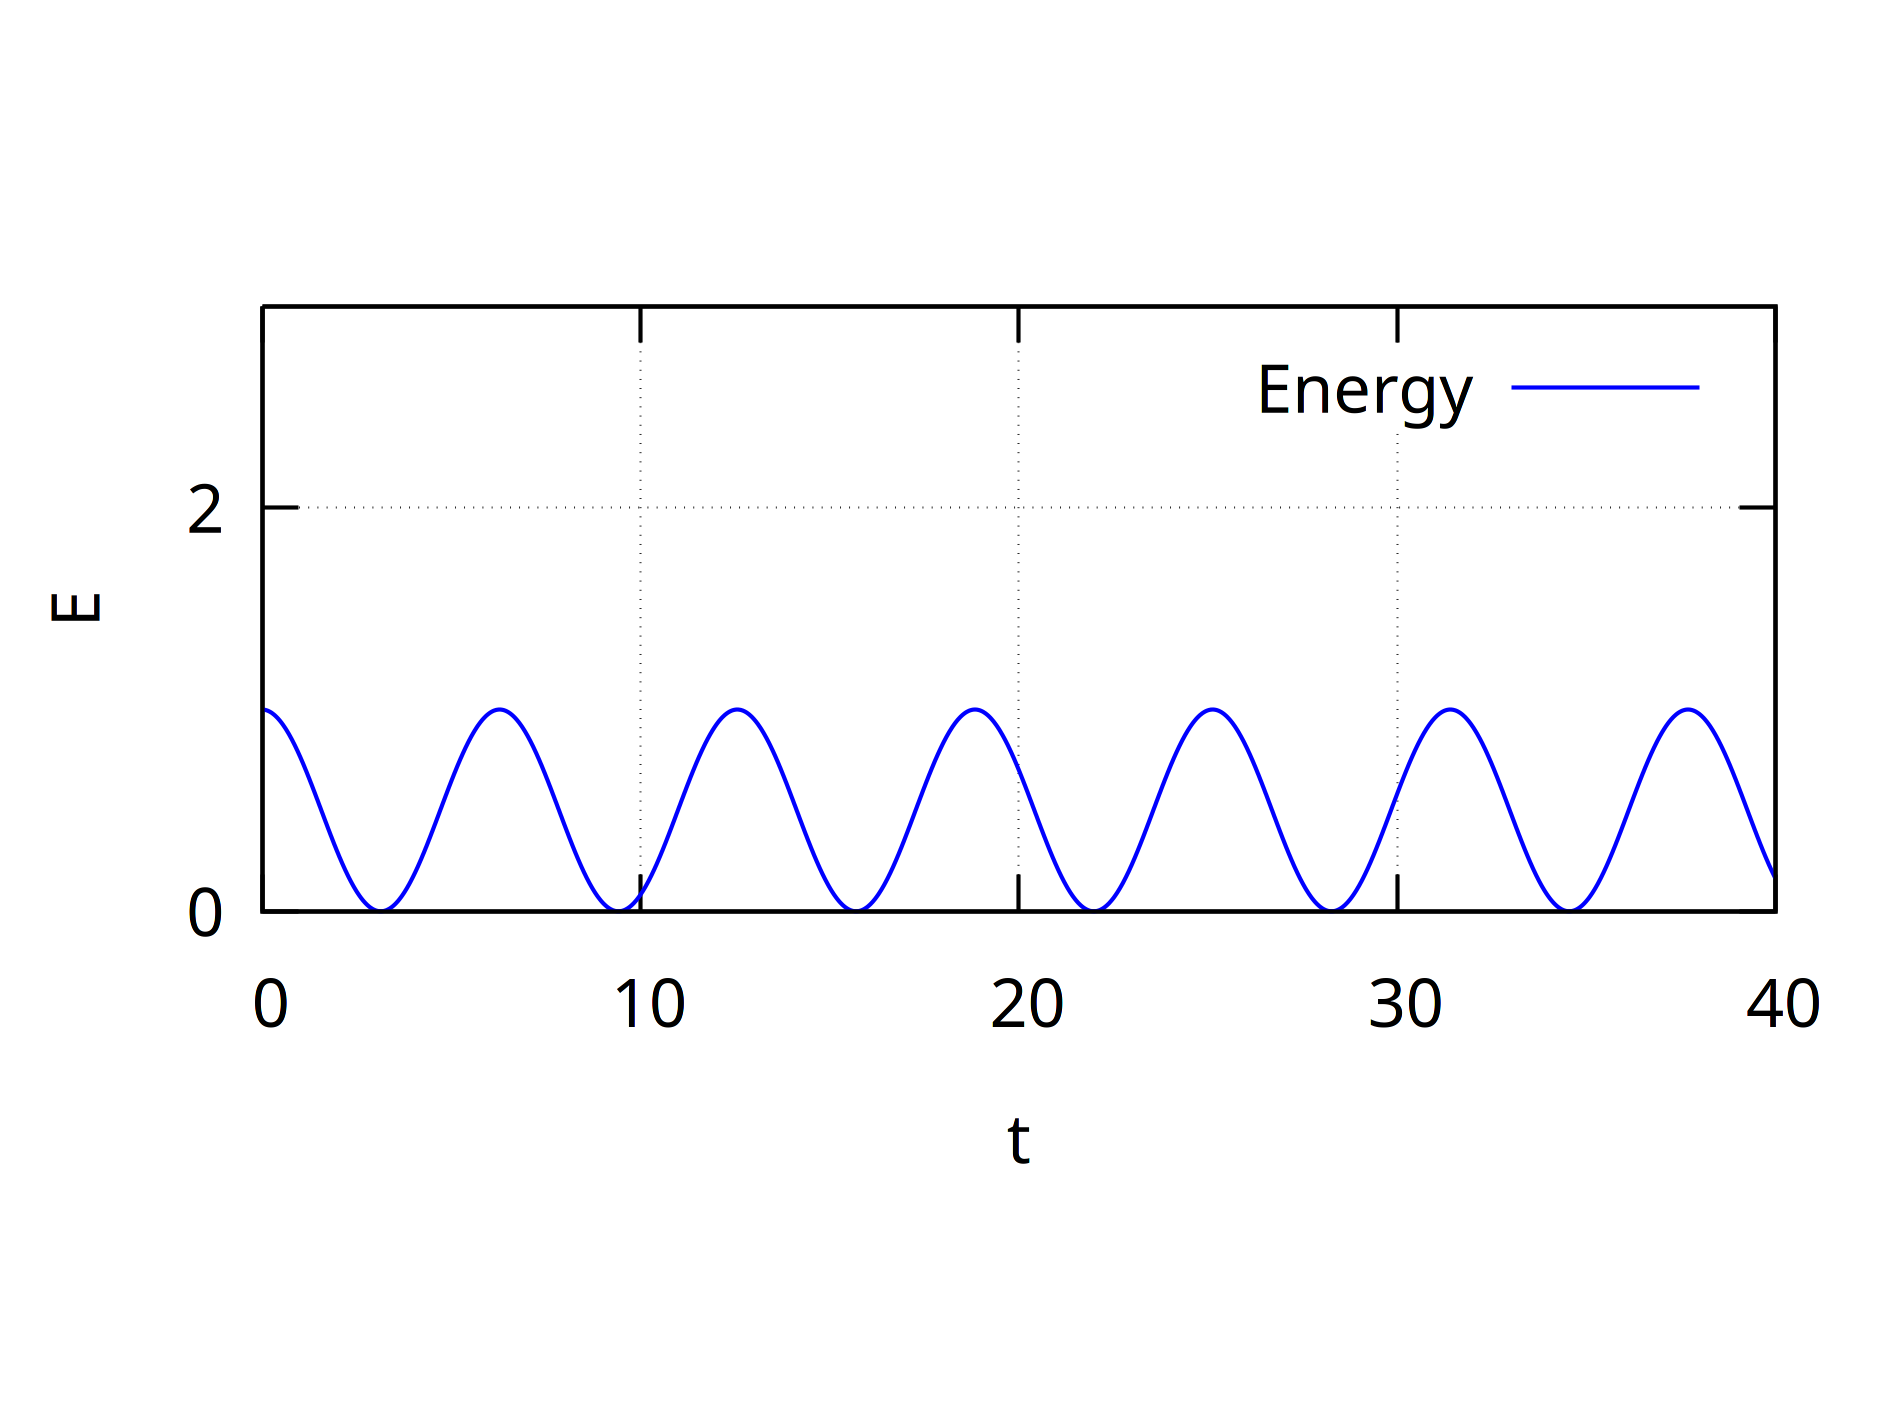
\includegraphics[width=.9\linewidth]{img/energia.png}  
  \caption{Energia}
\end{subfigure}
\caption{ExB Drift}
\end{figure}%
Si puó notare come la particella non abbia un guadagno netto di energia cinetica. Lo possiamo spiegare grazie alla derivazione della sezione precedente: se ci spostiamo in un sistema di riferimento che si muove con $\mathbf{v_d}$ annulliamo il campo $\mathbf{E}$, per cui la particella interagisce soltanto con $\mathbf{B}$. $\mathbf{B}$ non compie lavoro sulla particella, infatti non modifica il modulo della velocitá ma soltanto la direzione. \\
Per essere piú precisi questo cambio di sistema di riferimento puó essere effettuato soltanto se l'invariante relativistico $E^2 - B^2 $ é conservato, per cui $ \|\mathbf{E}\| < \|\mathbf{B}\|$. \\
Se $ \|\mathbf{E}\| > \|\mathbf{B}\|$ l'invariante non é piú conservato e non posso effettuare questo cambio di sistema di riferimento.


\end{document}
